% Options for packages loaded elsewhere
\PassOptionsToPackage{unicode}{hyperref}
\PassOptionsToPackage{hyphens}{url}
\PassOptionsToPackage{dvipsnames,svgnames,x11names}{xcolor}
%
\documentclass[
]{report}

\usepackage{amsmath,amssymb}
\usepackage{iftex}
\ifPDFTeX
  \usepackage[T1]{fontenc}
  \usepackage[utf8]{inputenc}
  \usepackage{textcomp} % provide euro and other symbols
\else % if luatex or xetex
  \usepackage{unicode-math}
  \defaultfontfeatures{Scale=MatchLowercase}
  \defaultfontfeatures[\rmfamily]{Ligatures=TeX,Scale=1}
\fi
\usepackage{lmodern}
\ifPDFTeX\else  
    % xetex/luatex font selection
\fi
% Use upquote if available, for straight quotes in verbatim environments
\IfFileExists{upquote.sty}{\usepackage{upquote}}{}
\IfFileExists{microtype.sty}{% use microtype if available
  \usepackage[]{microtype}
  \UseMicrotypeSet[protrusion]{basicmath} % disable protrusion for tt fonts
}{}
\makeatletter
\@ifundefined{KOMAClassName}{% if non-KOMA class
  \IfFileExists{parskip.sty}{%
    \usepackage{parskip}
  }{% else
    \setlength{\parindent}{0pt}
    \setlength{\parskip}{6pt plus 2pt minus 1pt}}
}{% if KOMA class
  \KOMAoptions{parskip=half}}
\makeatother
\usepackage{xcolor}
\setlength{\emergencystretch}{3em} % prevent overfull lines
\setcounter{secnumdepth}{-\maxdimen} % remove section numbering
% Make \paragraph and \subparagraph free-standing
\makeatletter
\ifx\paragraph\undefined\else
  \let\oldparagraph\paragraph
  \renewcommand{\paragraph}{
    \@ifstar
      \xxxParagraphStar
      \xxxParagraphNoStar
  }
  \newcommand{\xxxParagraphStar}[1]{\oldparagraph*{#1}\mbox{}}
  \newcommand{\xxxParagraphNoStar}[1]{\oldparagraph{#1}\mbox{}}
\fi
\ifx\subparagraph\undefined\else
  \let\oldsubparagraph\subparagraph
  \renewcommand{\subparagraph}{
    \@ifstar
      \xxxSubParagraphStar
      \xxxSubParagraphNoStar
  }
  \newcommand{\xxxSubParagraphStar}[1]{\oldsubparagraph*{#1}\mbox{}}
  \newcommand{\xxxSubParagraphNoStar}[1]{\oldsubparagraph{#1}\mbox{}}
\fi
\makeatother


\providecommand{\tightlist}{%
  \setlength{\itemsep}{0pt}\setlength{\parskip}{0pt}}\usepackage{longtable,booktabs,array}
\usepackage{calc} % for calculating minipage widths
% Correct order of tables after \paragraph or \subparagraph
\usepackage{etoolbox}
\makeatletter
\patchcmd\longtable{\par}{\if@noskipsec\mbox{}\fi\par}{}{}
\makeatother
% Allow footnotes in longtable head/foot
\IfFileExists{footnotehyper.sty}{\usepackage{footnotehyper}}{\usepackage{footnote}}
\makesavenoteenv{longtable}
\usepackage{graphicx}
\makeatletter
\newsavebox\pandoc@box
\newcommand*\pandocbounded[1]{% scales image to fit in text height/width
  \sbox\pandoc@box{#1}%
  \Gscale@div\@tempa{\textheight}{\dimexpr\ht\pandoc@box+\dp\pandoc@box\relax}%
  \Gscale@div\@tempb{\linewidth}{\wd\pandoc@box}%
  \ifdim\@tempb\p@<\@tempa\p@\let\@tempa\@tempb\fi% select the smaller of both
  \ifdim\@tempa\p@<\p@\scalebox{\@tempa}{\usebox\pandoc@box}%
  \else\usebox{\pandoc@box}%
  \fi%
}
% Set default figure placement to htbp
\def\fps@figure{htbp}
\makeatother

\usepackage{booktabs}
\usepackage{caption}
\usepackage{longtable}
\usepackage{colortbl}
\usepackage{array}
\usepackage{anyfontsize}
\usepackage{multirow}
\usepackage{titling}
\pretitle{\begin{center}\LARGE\bfseries}
\posttitle{\end{center}}
\preauthor{\begin{center} \large}
\postauthor{\end{center}}
\predate{\begin{center}\large}
\postdate{\begin{figure}[h] \centering 
\includegraphics[width=0.8\textwidth]{images/I1.png} \end{figure} \url{www.example.com} \end{center}}
\makeatletter
\@ifpackageloaded{caption}{}{\usepackage{caption}}
\AtBeginDocument{%
\ifdefined\contentsname
  \renewcommand*\contentsname{Table of contents}
\else
  \newcommand\contentsname{Table of contents}
\fi
\ifdefined\listfigurename
  \renewcommand*\listfigurename{List of Figures}
\else
  \newcommand\listfigurename{List of Figures}
\fi
\ifdefined\listtablename
  \renewcommand*\listtablename{List of Tables}
\else
  \newcommand\listtablename{List of Tables}
\fi
\ifdefined\figurename
  \renewcommand*\figurename{Figure}
\else
  \newcommand\figurename{Figure}
\fi
\ifdefined\tablename
  \renewcommand*\tablename{Table}
\else
  \newcommand\tablename{Table}
\fi
}
\@ifpackageloaded{float}{}{\usepackage{float}}
\floatstyle{ruled}
\@ifundefined{c@chapter}{\newfloat{codelisting}{h}{lop}}{\newfloat{codelisting}{h}{lop}[chapter]}
\floatname{codelisting}{Listing}
\newcommand*\listoflistings{\listof{codelisting}{List of Listings}}
\makeatother
\makeatletter
\makeatother
\makeatletter
\@ifpackageloaded{caption}{}{\usepackage{caption}}
\@ifpackageloaded{subcaption}{}{\usepackage{subcaption}}
\makeatother

\usepackage{bookmark}

\IfFileExists{xurl.sty}{\usepackage{xurl}}{} % add URL line breaks if available
\urlstyle{same} % disable monospaced font for URLs
% Make links footnotes instead of hotlinks:
\DeclareRobustCommand{\href}[2]{#2\footnote{\url{#1}}}
\hypersetup{
  pdftitle={Technical Report: A Case Study in Apple},
  pdfauthor={Marius Helten},
  colorlinks=true,
  linkcolor={blue},
  filecolor={Maroon},
  citecolor={Blue},
  urlcolor={Blue},
  pdfcreator={LaTeX via pandoc}}


\title{Technical Report: A Case Study in Apple}
\author{Marius Helten}
\date{2025-02-09}

\begin{document}
\maketitle


\section{Introduction}\label{introduction}

Food and perishable goods are critical products in societies worldwide
and provide great challenges for industry and consumers alike. The
quality of the goods is constantly changing during the lifetime of the
products, and many precautions have to be taken in order to control and
maintain the quality; this includes proper harvest and storage, cooling
chains, and other measures. Therefore a quick and easy way of
classifying the quality of individual items is a major concern.

In the following report, we present a comparative study of a supervised
learning classification problem with an approach from deep learning and
a comparative approach from ``traditional'' machine learning. The
central question is if, based on the available data, we can create
neural network models that can reliably predict the quality of an apple
based on its features.

For the training and evaluation of the models, we will use a dataset
that was generously provided by an anonymous American agriculture
\href{https://www.kaggle.com/datasets/nelgiriyewithana/apple-quality}{company}
with 4000 observations and the following variables, Unique ID, Size,
Weight, Sweetness, Crunchiness, Juiciness, Ripeness, Acidity and
Quality.

\section{Analysis}\label{analysis}

\subsection{Exploratory Data Analysis}\label{exploratory-data-analysis}

\subsubsection{Single Variables and their
Distributions}\label{single-variables-and-their-distributions}

We will start off with an exploratory analysis of the dataset and take a
look at the individual distributions of the features. A model can only
be as good as the data it is based on.

It is very interesting that our dataset contains a sample that is
distributed almost perfectly 50/50 into good and bad apples in a uniform
distribution, so it seems to be more than just a few bad apples. This at
least hints at a stratified sample in the selection of our data.\\
We also do not have any information about the quality classification
itself, so we do not know how the category was constructed and why
apples were classified either way. This will have a big influence on our
further analysis, though, since we are trying to classify for exactly
these two categories.

\begin{table}
\caption*{
{\large Table 1: Summary Statistics of Dataset Variables}
} 
\fontsize{12.0pt}{14.4pt}\selectfont
\begin{tabular*}{\linewidth}{@{\extracolsep{\fill}}lrr}
\toprule
Variable & Mean & SD \\ 
\midrule\addlinespace[2.5pt]
A\_id & 1999.50 & 1154.84 \\ 
Size & -0.50 & 1.93 \\ 
Weight & -0.99 & 1.60 \\ 
Sweetness & -0.47 & 1.94 \\ 
Crunchiness & 0.99 & 1.40 \\ 
Juiciness & 0.51 & 1.93 \\ 
Ripeness & 0.50 & 1.87 \\ 
Acidity & 0.08 & 2.11 \\ 
Quality & 0.50 & 0.50 \\ 
\bottomrule
\end{tabular*}
\end{table}

Statistical measures like mean and standard deviation give us a first
impression as to what we are dealing with. The A\_id do not provide us
with any useful information for our problem and will be excluded from
here on. The other features have some variance and also different means,
and so might provide us with useful variance.

The box plots (1.a) confirm the impression from the statistical
measures. We can see that there are differences between the centers of
the distribution of the attributes for each of our quality categories;
the areas where the distributions don't overlap are the areas where we
can distinguish between the quality categories.

The variables are all unimodal normal distributions, which is pretty
natural for variables such as size and weight. Also, some outliers are
part of the distributions (points in the box plots); these were kept due
to a limited amount of data.

\begin{figure}[h]
    \begin{subfigure}{0.45\textwidth} % Adjust width as needed
        \centering
        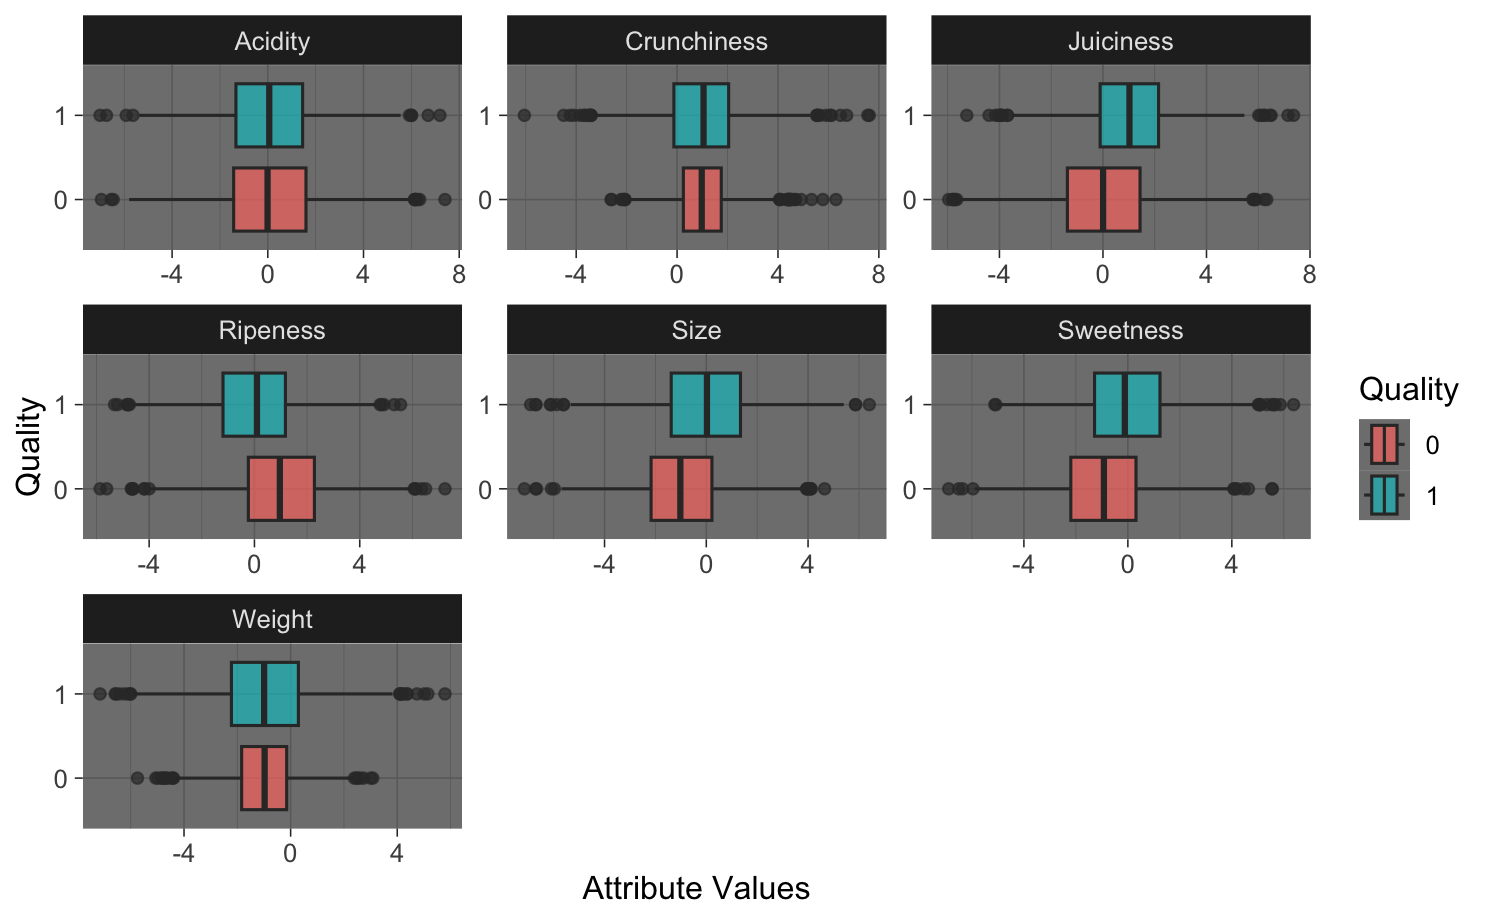
\includegraphics[width=\textwidth]{images/BP1.png}
        \caption{Box Plots}
        \label{fig:scree_plot}
    \end{subfigure}
    \hfill % This adds space between the two subfigures
    \begin{subfigure}{0.45\textwidth} % Adjust width as needed
        \centering
        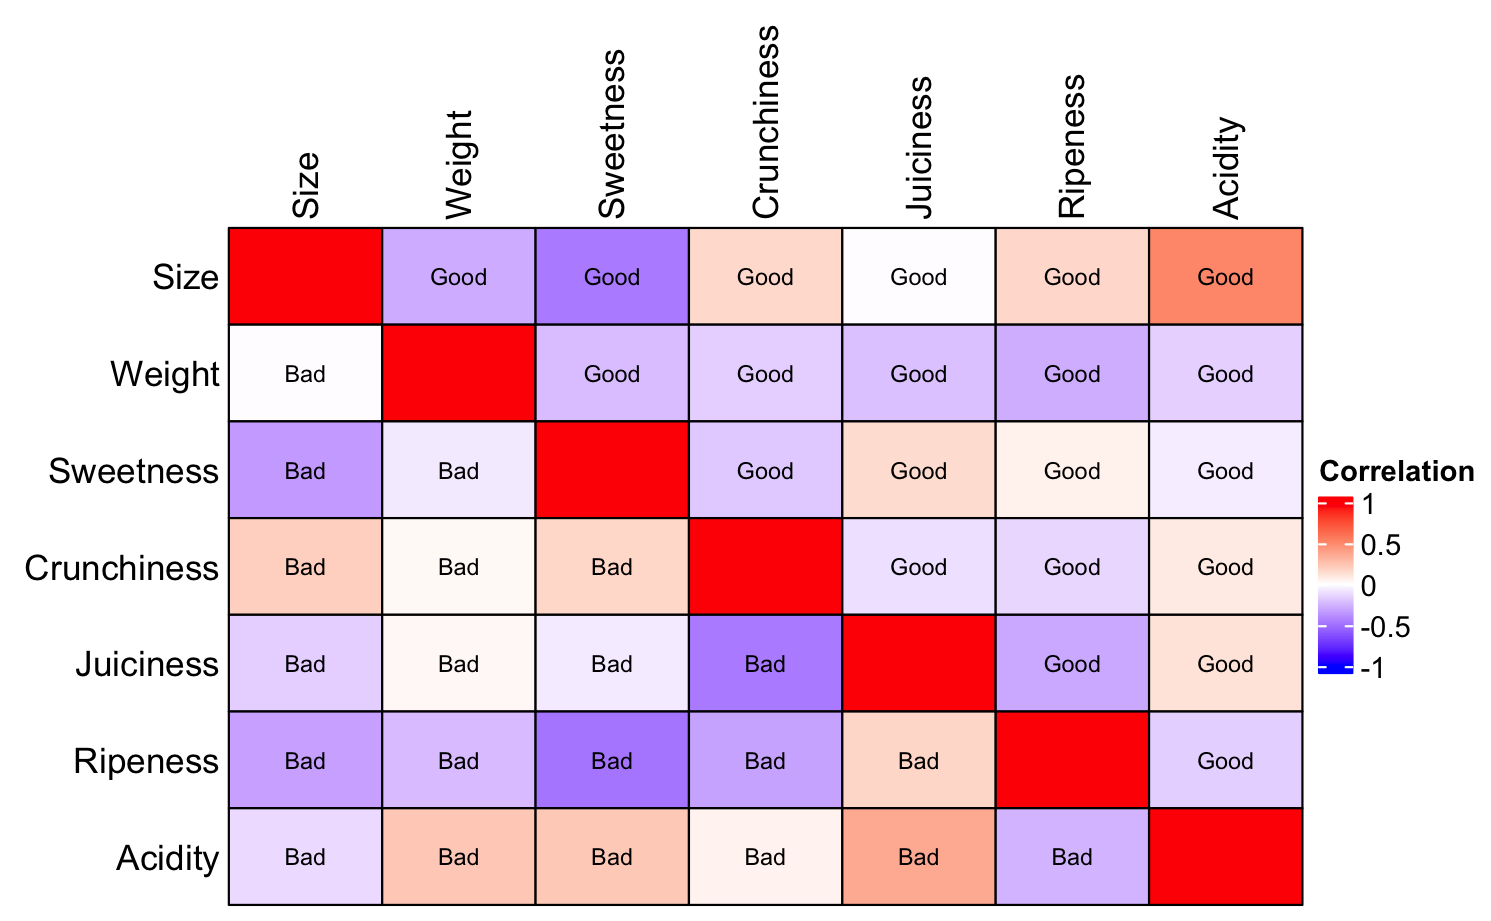
\includegraphics[width=\textwidth]{images/HM1.png}
        \caption{Correlation Heatmap}
        \label{fig:pca_result}
    \end{subfigure}
    \caption{Single Distributions and Pairwise Correlations for Features}
    \label{fig:pca_combined}
\end{figure}

\subsubsection{Attribute Correlation
Heatmap}\label{attribute-correlation-heatmap}

The next step after looking at single attributes is to look at more
attributes at the same time. (1.b) The attributes on the diagonal are
perfectly correlated with each other. The other blue and red fields
provide attribute combinations that increase together or go in opposite
directions. Also fascinating are pairs where the bad and good quality
have an opposite signed correlation because it suggests that the
relationship between those features will flip depending on the quality
category.

\subsubsection{PCA - Principal Component
Analysis}\label{pca---principal-component-analysis}

Working with high-dimensional data introduces significant challenges, as
representation and analysis become increasingly complex in such spaces.
Specialized methods exist to address these challenges. A good example is
the PCA, a technique that generates a set of principal components
ordered by their explanatory strength. These components capture the
maximum variance in the data, effectively providing a lower-dimensional
representation of the high-dimensional dataset while preserving its most
critical information. The PCA Loadings (2) shows how much influence each
attribute has and also infers about relations between them; for example,
ripeness and acidity seem to have an opposing relation, and sweetness
and juiciness, as well as crunchiness and size, seem to be similar.

\begin{figure}[h]
  \centering
  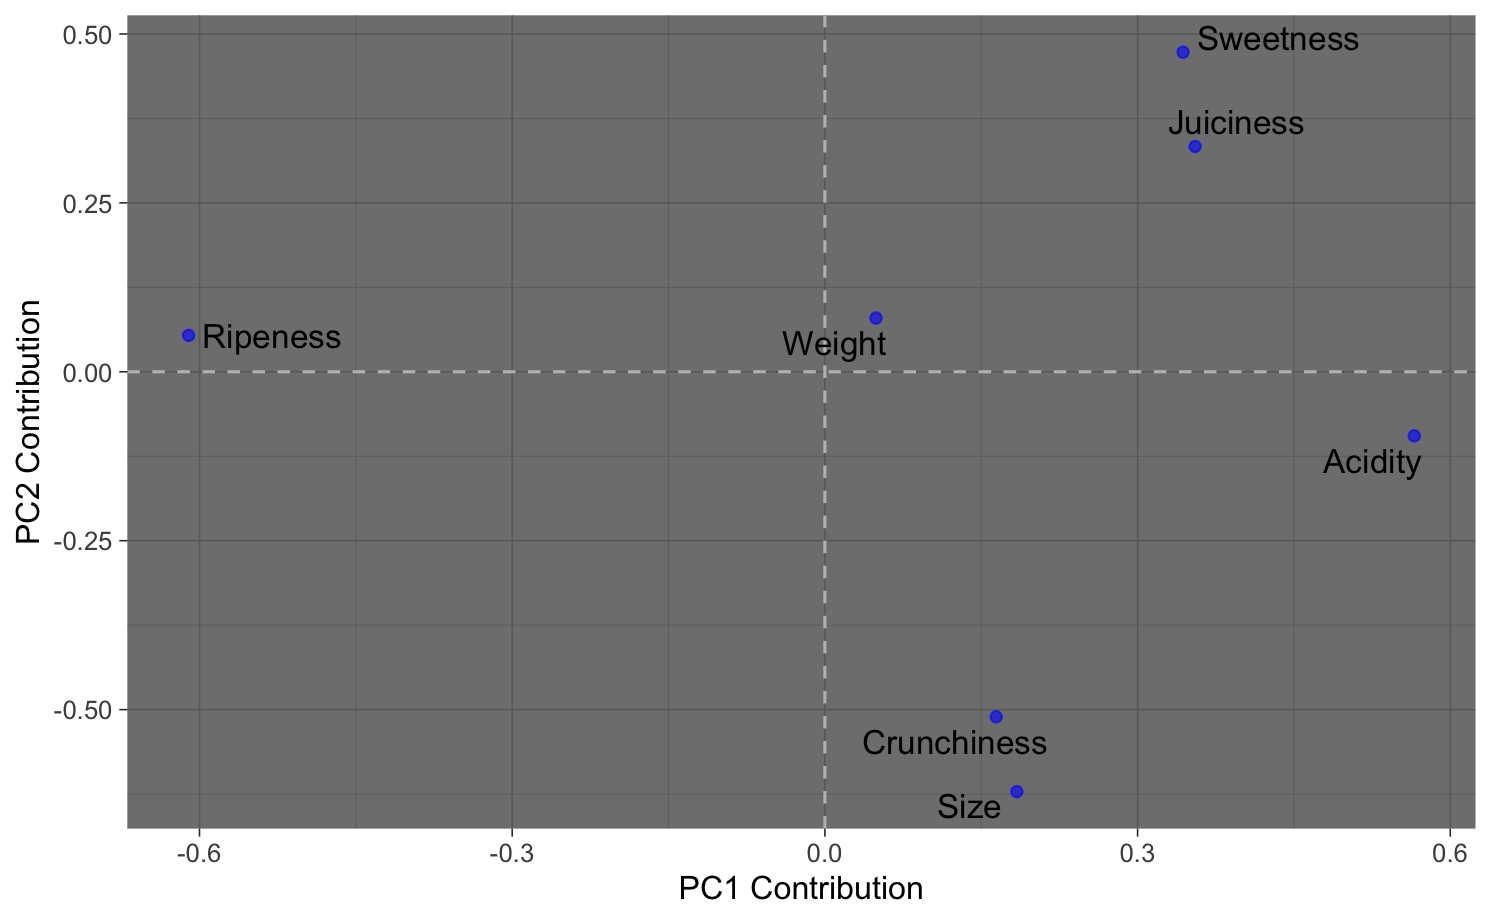
\includegraphics[width=0.6\textwidth]{images/PCA3.png}
  \caption{PCA Loadings for PC1 and PC2}
  \label{fig:pca_combined}
\end{figure}

\subsection{Feature Selection and Data
Preprocessing}\label{feature-selection-and-data-preprocessing}

The dataset contains only limited amounts of data; therefore, all
features were kept, except for the unique ID's, since they provide no
relevant information and might compromise the training of the models.
The numerical features were scaled through z-standardization, and the
target variable of quality was turned into a dummy variable (0: Bad / 1:
Good).

\section{Methods}\label{methods}

\subsection{Neural Network}\label{neural-network}

\subsubsection{Architecture}\label{architecture}

The neural network is a feed-forward neural network (also known as a
multi-layer perceptron, or MLP) designed for a binary classification
task. For most on the neural net, we use the very efficient ReLU
Rectified Linear Unit Activation Function. In the output layer the
Sigmoid function gives us logarithmic odds, which we can transform into
a binary classification. The dropout rate prevents over-fitting by
knocking out random neurons on each pass. The model architecture for the
hidden layers was chosen based on good practices and trial and error in
the construction phase.

\begin{enumerate}
\def\labelenumi{\arabic{enumi}.}
\item
  \textbf{Input Layer}:

  \begin{itemize}
  \tightlist
  \item
    Passes the input through a fully connected (dense) layer with 1024
    units.
  \item
    Applies the ReLU activation function
  \end{itemize}
\item
  \textbf{Hidden Layers 1, 2, 3}:

  \begin{itemize}
  \item
    A fully connected layer with 1024/512/256 input units and
    521/256/128 output units.
  \item
    Applies the ReLU activation function
  \item
    Applies a dropout rate of 10\% (1 \& 2): share of neurons in that
    layer will be randomly turned off in each training step
  \end{itemize}
\item
  \textbf{Output Layer}:

  \begin{itemize}
  \item
    A fully connected layer with 128 input units and 1 output unit.
  \item
    Applies the sigmoid activation function to produce a probability
    score between 0 and 1
  \end{itemize}
\end{enumerate}

\subsubsection{Training and Learning}\label{training-and-learning}

For the training of the neural network model we use the
binary-classification error loss function and the Adam-optimizer with a
fixed learning rate(0.001) and weight decay (0.01). We trained the model
with batch of sizes of 32 observations for efficiency and stability. The
model Quality is tested with a 5-fold cross validation. Note that k-fold
cross-validation was used to evaluate the model design, not a particular
training by re-train the model of the same design. After a certain
period without improvement, the learning is stopped.

\subsection{Random Forest}\label{random-forest}

As comparison for our model we used a Random Forest classifier it is an
ensemble learning method. It builds multiple decision trees during
training and merges their outputs to improve the overall performance and
robustness of the model. The models was validated with the 5-fold cross
validation.

\section{Results}\label{results}

The first graph (3) shows the neural network model during training. We
can see very well that as training progresses, the loss of the model
through false predictions gets smaller, while the accuracy rises through
correct predictions. The minimal divergence between training and
validation results for loss and accuracy is a good sign, as this shows
our model is not over-fitting to the training data. The longer training
continues, the more we run the risk of adapting our model too much to
the training data (over-fitting); this is why we stop learning. We can
see very well the diminishing returns as training progresses. We can
also see the cross-fold validation, since in each iteration the model is
trained again from scratch.

\begin{figure}[h]
  \centering
  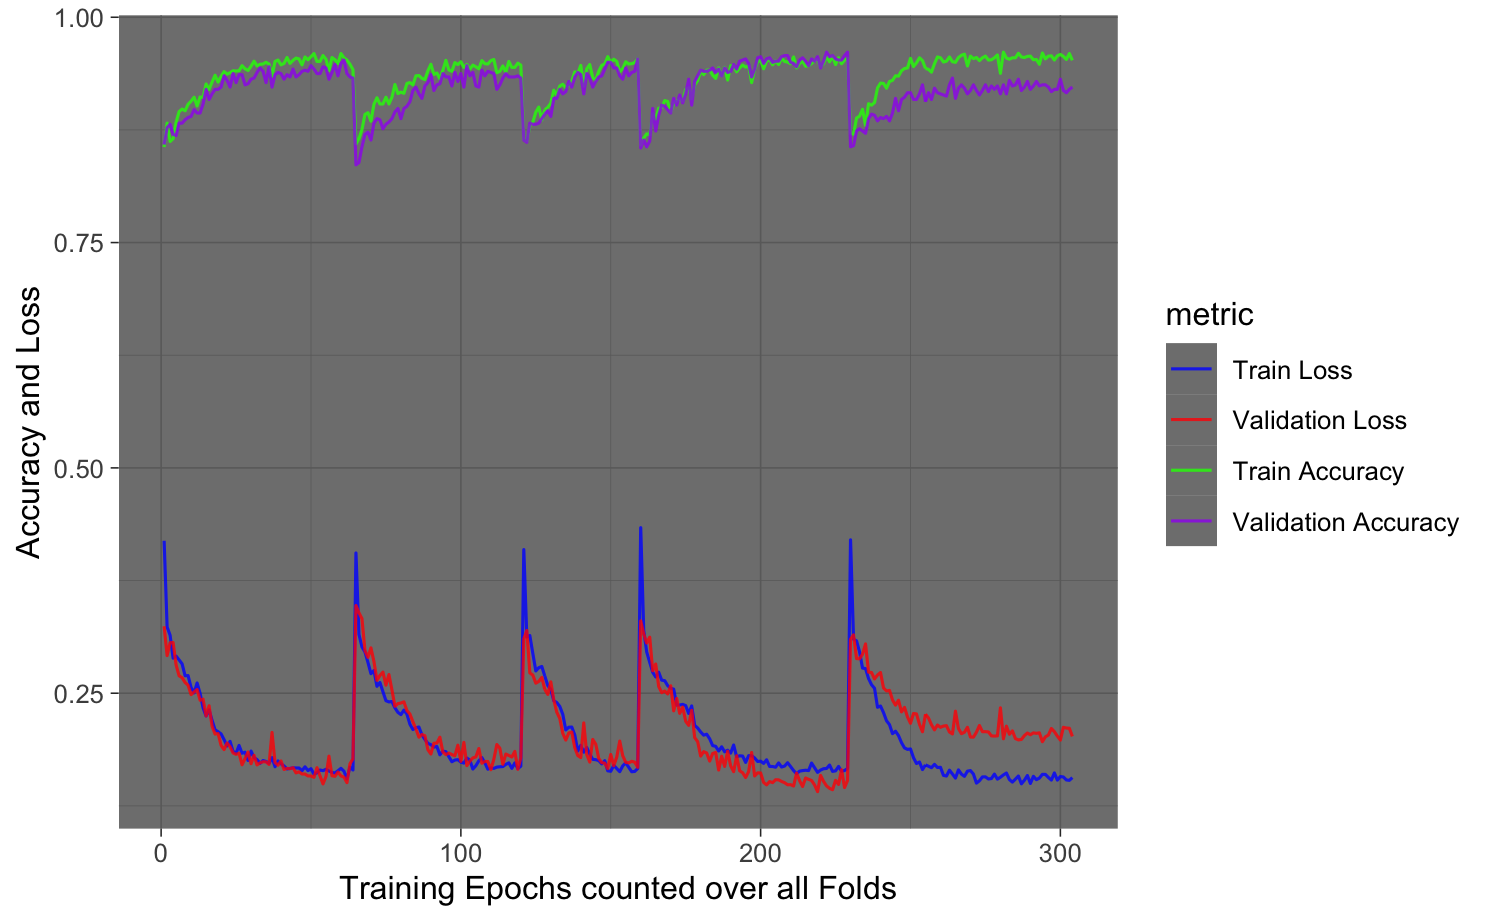
\includegraphics[width=0.6\textwidth]{images/NN1.png}
  \caption{Loss and Accuracy of Neural Network during Training}
  \label{fig:pca_combined}
\end{figure}

Below (4.a), we can see all the different fields of the confusion
matrix. If we wanted to optimize the average quality of our sold apples
without caring about waste, we would choose a model with as few false
positives as possible, while tolerating some bad apples to increase
throughput would lower false negatives, so it heavily depends on the use
case, we maximized accuracy (True-Positives).

The neighboring graph (4.b) shows the 95\% confidence interval for the
accuracy of the neural network and random forest, the CI was calculated
by k-fold cross-validation. We can see that the neural network
outperforms the other approaches, with an accuracy of close to 94\%.
Taking a look at other evaluative metrics (5.a) for the machine learning
models, this impression gets confirmed. The neural network is the
stronger across the board for all metrics. Including Recall, F1 Balanced
Accuracy, Specificity and Precision.

\begin{figure}[h]
    \begin{subfigure}{0.45\textwidth} % Adjust width as needed
        \centering
        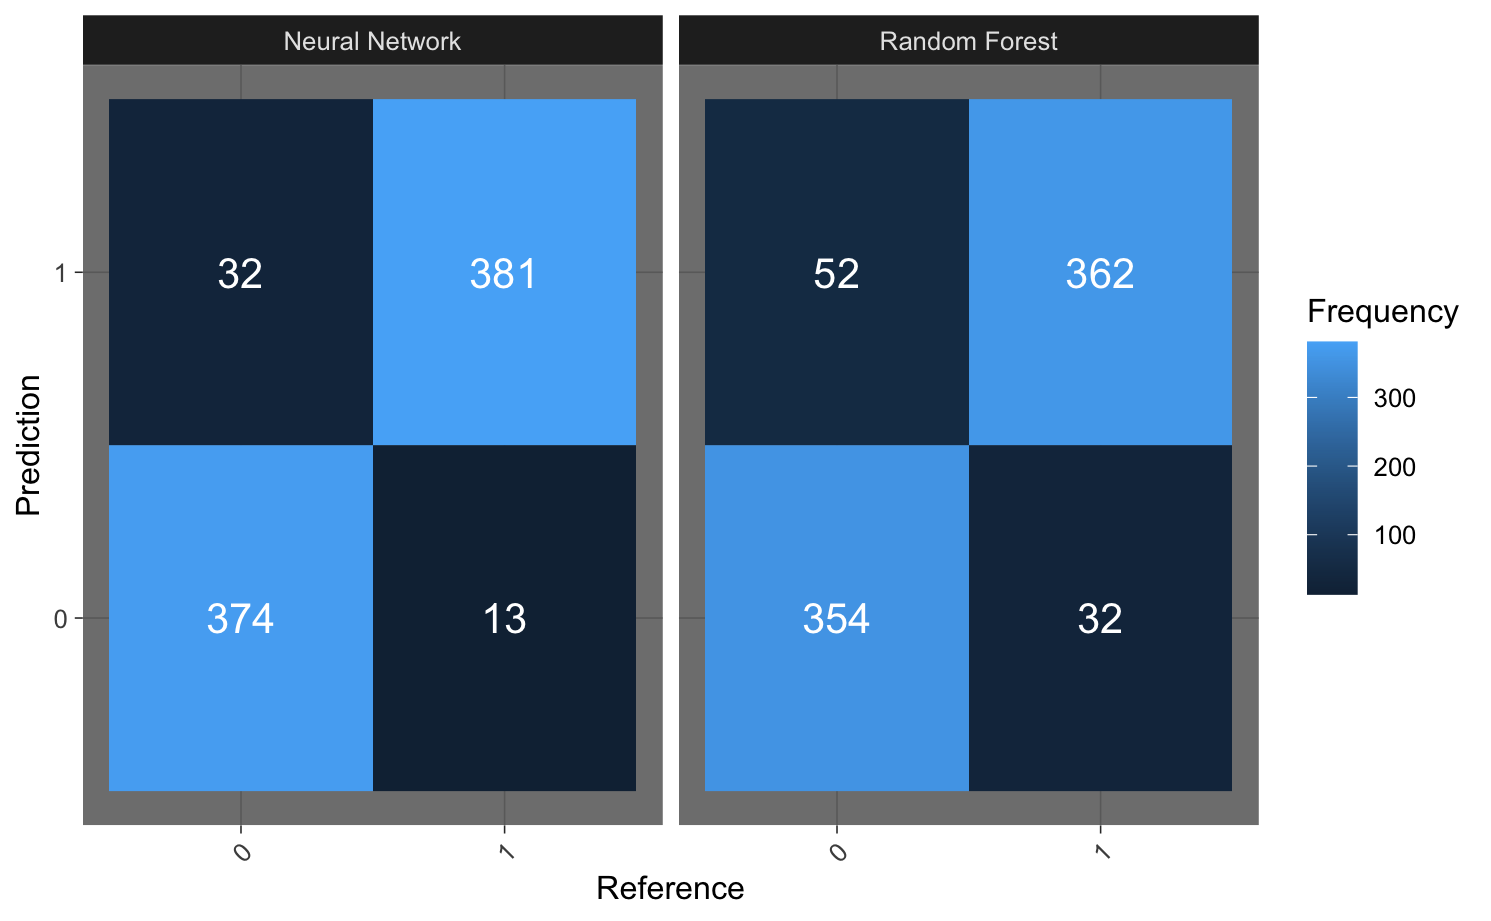
\includegraphics[width=\textwidth]{images/NNRF4.png}
        \caption{Confusion Matrices for Predictions}
        \label{fig:scree_plot}
    \end{subfigure}
    \hfill % This adds space between the two subfigures
    \begin{subfigure}{0.45\textwidth} % Adjust width as needed
        \centering
        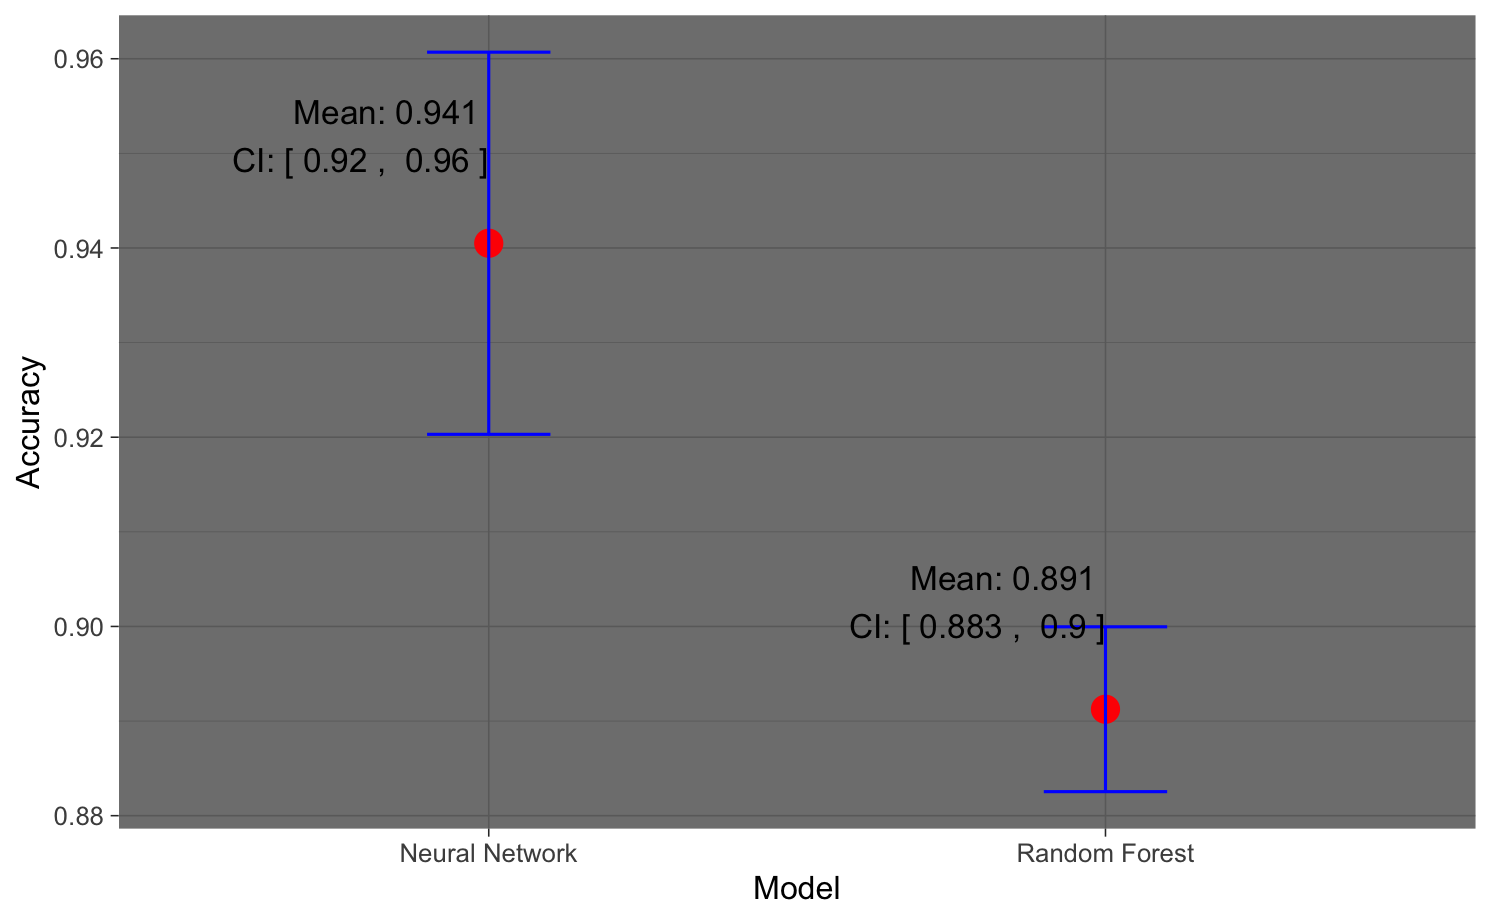
\includegraphics[width=\textwidth]{images/NNRF2.png}
        \caption{Model Accuracy with Confidence Intervall}
        \label{fig:pca_result}
    \end{subfigure}
    \caption{Model Evaluation and Comparison I}
    \label{fig:pca_combined}
\end{figure}

The following graph (6.b) shows the precision-recall curve. In our case,
the curve only starts to dip at the very end, which is good because it
means we are not losing F1 score while moving the threshold between
precision and recall. The closer the AUC is to 1, the better the model
distinguishes between positive and negative cases. We can also see some
differences between the model.

\begin{figure}[h]
    \begin{subfigure}{0.45\textwidth} % Adjust width as needed
        \centering
        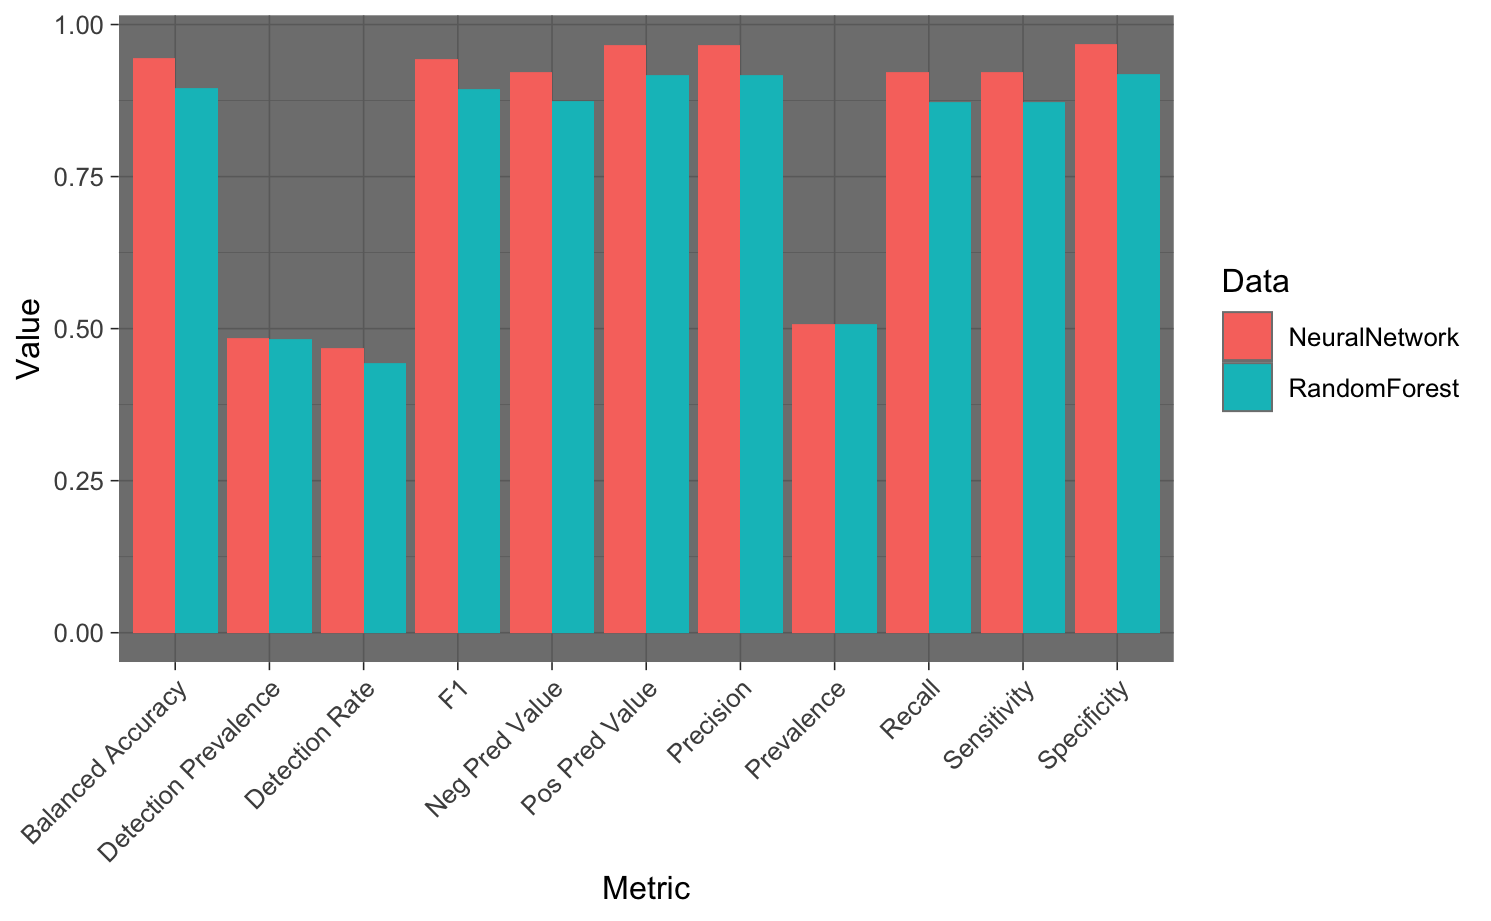
\includegraphics[width=\textwidth]{images/NNRF1.png}
        \caption{Evaluative Metrics}
        \label{fig:scree_plot}
    \end{subfigure}
    \hfill % This adds space between the two subfigures
    \begin{subfigure}{0.45\textwidth} % Adjust width as needed
        \centering
        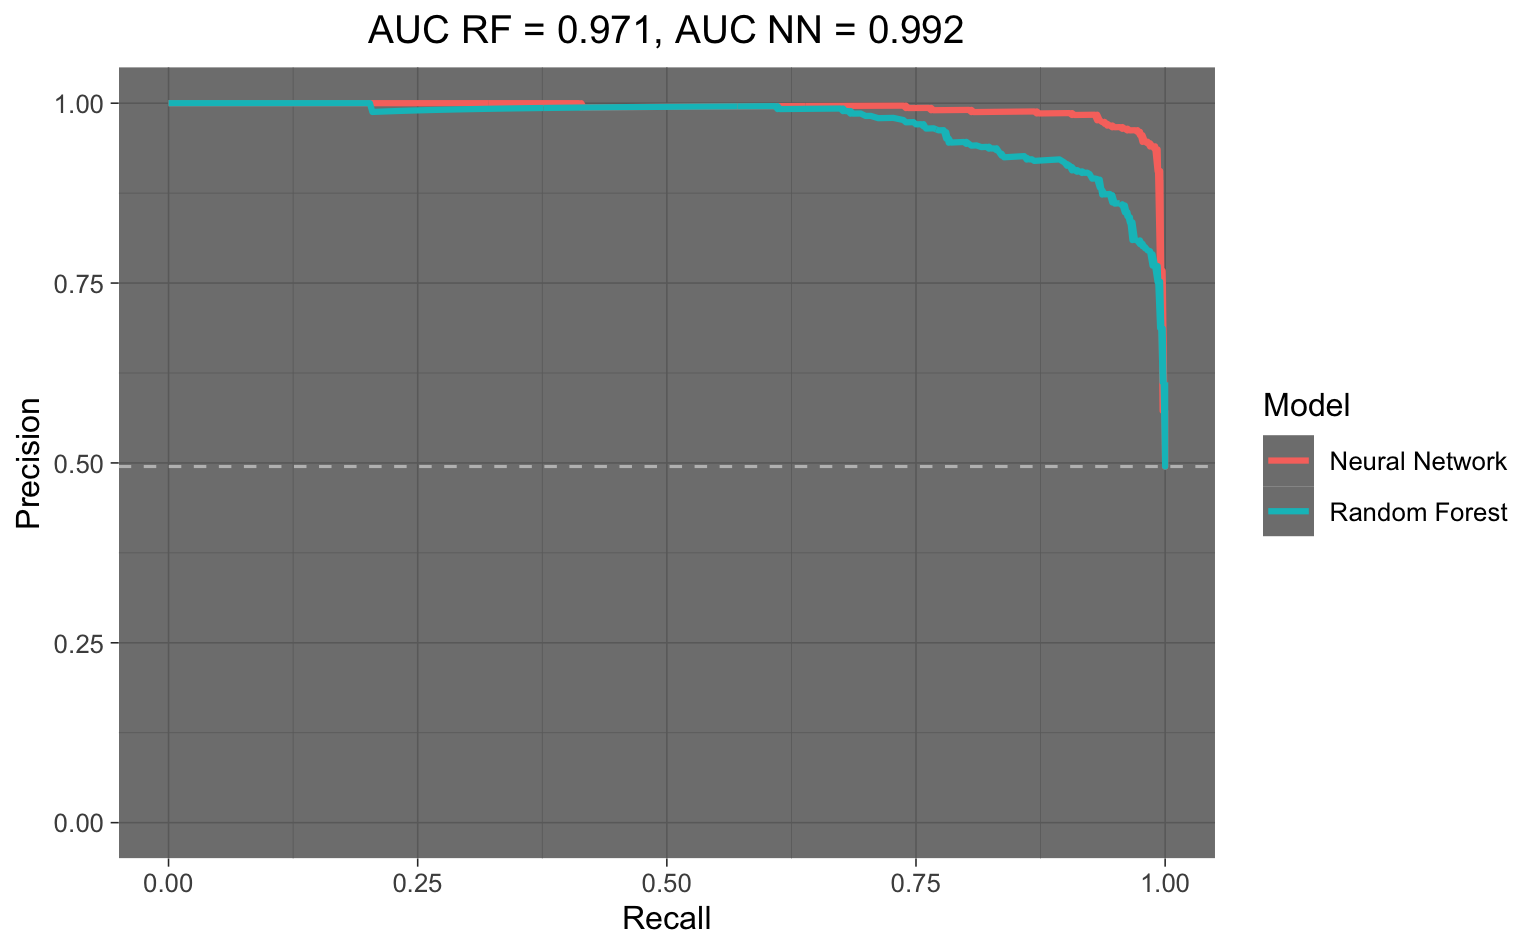
\includegraphics[width=\textwidth]{images/NNRF3.png}
        \caption{Precision-Recall Curve with AUC}
        \label{fig:pca_result}
    \end{subfigure}
    \caption{Model Evaluation and Comparison II}
    \label{fig:pca_combined}
\end{figure}

\section{Reflection}\label{reflection}

The deep learning approach using a neural network proved to be useful
and practical. While the other methods achieved respectable outcomes,
the neural network's performance was superior. The computational costs
were very limited during the analysis, but might prove problematic
during scale-up. The high number of parameters made tuning challenging.
Here a more comprehensive tuning approach could give even better
results.

A key drawback of neural networks is the lack of information; unlike
methods such as PCA or decision trees, we cannot ascertain the relative
importance of features, which can be important to explain the decision.
Additionally, the validation and training were based on the current
dataset, more data would lead to a more robust evaluation and training
process.

Concrete implementation goals and setting are essential when selecting
the best model for a task. For instance, assessing if an apple is
poisonous or edible vs.~how it looks, is some cases might tolerate
higher error rates in our classification than in others. Nonetheless,
this example highlights the potential of data analysis and deep learning
methods to address complex problems and the practicality of obtaining
results with them.




\end{document}
